% Template made by the IEEE Computational Intelligence Society, which provided the current LaTeX template.
% Use pdflatex or latex + dvips + ps2pdf to produce a PDF.
% http://www.ieee.org/conferences_events/conferences/publishing/templates.html
\documentclass[conference]{IEEEtran}
\IEEEoverridecommandlockouts
% The preceding line is only needed to identify funding in the first footnote. If that is unneeded, please comment it out.

%% Add packages and define personal macros here, but ensure that they do not
%% interfere with the fonts and page layout. FIXME Do not add hyperlinks.
%% ------------------ Beginning of header ------------------
%% AMS maths and others
\usepackage{amsmath,amsfonts,amssymb}
\usepackage{bbm,bm}
% \usepackage{cite}
\usepackage{textcomp}
\usepackage{xcolor}
% \def\BibTeX{{\rm B\kern-.05em{\sc i\kern-.025em b}\kern-.08em
%     T\kern-.1667em\lower.7ex\hbox{E}\kern-.125emX}}
%% Reference
\usepackage[nameinlink]{cleveref} % \cref{} command, tips from http://tex.stackexchange.com/a/205133/97964
%% Source code
\usepackage{graphicx}

% The paper has 6 pages, has a paper size of 8.5x11 inches (letter), is formatted in 2 columns, with a gutter of 0.16 inches (smallest on pg. 1), margins are 0.67 (L) x 0.67 (R) x 0.69 (T) x 1.02 (B) inches, using PDF version 1.5, created by TeX.

\usepackage[letterpaper]{geometry}
\geometry{
left=0.67in,
right=0.67in,
top=0.71in,
bottom=1.02in
}

\usepackage[export]{adjustbox}  % https://tex.stackexchange.com/a/91580/

\usepackage{algorithm2e}  % https://en.wikibooks.org/wiki/LaTeX/Algorithms#Typesetting_using_the_algorithm2e_package
%% Various theorems, numbered by section (required amsthm)
\usepackage{amsthm}
\theoremstyle{plain}  % Plain style for theorem, defn, lemma, proposition, corollary
\newtheorem{theorem}{Theorem}[section]
\newtheorem{lemma}[theorem]{Lemma}
%% Macros
\renewcommand{\P}[0]{\mathbb{P}}
\newcommand{\E}[0]{\mathbb{E}}
% Shortcuts
\newcommand{\ie}{\emph{i.e.}}
\newcommand{\iid}{\emph{i.i.d.}}
\newcommand{\eg}{\emph{e.g.}}
\newcommand{\UCB}[0]{$\mathrm{UCB}$}
\newcommand{\kl}[0]{\ensuremath{\mathrm{kl}}}
\newcommand{\klUCB}[0]{$\mathrm{kl}$-$\mathrm{UCB}$}
\newcommand{\Aggr}[0]{\textbf{Aggregator}}
\newcommand{\ExpQ}[0]{\textbf{Exp4}}
\newcommand{\CORRAL}[0]{\textbf{CORRAL}}
\newcommand{\LearnExp}[0]{\textbf{LearnExp}}
\newcommand{\Alg}[0]{\mathcal{A}}

\newcommand{\hr}{\begin{center}\rule{0.5\linewidth}{\linethickness}\end{center}}

\makeatletter
\newcommand{\removelatexerror}{\let\@latex@error\@gobble}  % From http://tex.stackexchange.com/a/82272/
\makeatother
%% ------------------ End of header ------------------

\title{Aggregation of Multi-Armed Bandits Learning \\
	   Algorithms for Opportunistic Spectrum Access
\thanks{
	This work is supported by the French National Research Agency (ANR) with the project BADASS,
	(\texttt{N ANR-16-CE40-0002}),
	the CNRS with the project PEPS8 BIO,
	% (\texttt{XXX XXX XXX XXX}), %
	the French Ministry of Research (MENESR) and ENS Paris-Saclay.}
}

\author{
Lilian Besson$^{1,2}$, Emilie Kaufmann$^{2}$ and Christophe Moy$^{3}$ \vspace{0.3cm} \\


$^1$ CentraleSup\'elec, IETR--SCEE, Cesson-S\'evign\'e, France, \texttt{Lilian.Besson@CentraleSupelec.fr} \\
$^2$ CNRS $\&$ CRIStAL, Univ. Lille 1, Inria SequeL, Lille, France, \texttt{Emilie.Kaufmann@Univ-Lille1.fr} \\
$^3$ University Rennes, CNRS, IETR -- UMR 6164, Rennes, France, \texttt{Christophe.Moy@Univ-Rennes1.fr}}
%	\IEEEauthorblockN{Lilian Besson\textsuperscript{$*$}}
%	SequeL \& SCEE Teams \\
%	\IEEEauthorblockA{\textit{CentraleSup{\'e}lec, campus of Rennes, IETR}, Rennes, France. \\
%	\texttt{{Lilian}.{Besson}{@}{CentraleSupelec}.{fr}}}
%\and
%	\IEEEauthorblockN{Christophe Moy}
%	SCEE Team \\
%	\IEEEauthorblockA{\textit{Universit{\'e} Rennes 1, IETR}, Rennes, France. \\
%	\texttt{{Christophe}.{Moy}{@}{Univ}-{Rennes1}.{fr}}}\\
% \and
%	\IEEEauthorblockN{Emilie Kaufmann}
%	SequeL Team \\
%	\IEEEauthorblockA{\textit{Inria Lille - Nord Europe, CRIStAL}, Lille, France. \\
%	\texttt{{Emilie}.{Kaufmann}{@}{Inria}.{fr}}}


\begin{document}

\maketitle

\begin{abstract}
	Multi-armed bandit algorithms have been recently studied and evaluated
	for Cognitive Radio (CR),
	especially in the context of Opportunistic Spectrum Access (OSA).
	% \cite{Zhao07,Jouini12}.
	Several solutions have been explored based on various models,
	but it is hard to exactly predict which could be the best for real-world conditions at every instants.
	Hence, expert aggregation algorithms can be useful to select \emph{on the run} the best algorithm for a specific situation.
	%
	Aggregation algorithms, such as \ExpQ{}
	dating back from 2002,
	% \cite{Auer02},
	have never been used for OSA learning,
	and we show that it appears empirically sub-efficient when applied to simple stochastic problems.
	%
	In this article, we present an improved variant, called \emph{\Aggr}.
	For synthetic OSA problems modeled as Multi-Armed Bandit (MAB) problems,
	% with Bernoulli-distributed arms,
	simulation results are presented to demonstrate its empirical efficiency.
	We combine classical algorithms, such as Thompson sampling, Upper-Confidence Bounds algorithms (\UCB{} and variants), and Bayesian or Kullback-Leibler UCB.
	%
	Our algorithm offers good performance compared to state-of-the-art algorithms
	(\ExpQ{}, \CORRAL{} or \LearnExp{}),
	% \cite{Agarwal16,Singla17}),
	and appears as a robust approach to select on the run the best algorithm for any stochastic MAB problem, being more realistic to real-world radio settings than any tuning-based approach.
	% Our proposal is empirically better than other state-of-the-art aggregation algorithms,
	% Theoretical analysis on its performance is left as a future work.
\end{abstract}

\begin{IEEEkeywords}
	cognitive radio, learning theory, robust aggregation algorithms, multi-armed bandits, reinforcement learning.
\end{IEEEkeywords}


% ----------------------------------------------------------------------
\section{Introduction}\label{seq:introduction}
% FIXME be quicker and shorter!

% - model: OSA as a Bernoulli MAB problem (PU, SU)
% Cognitive Radio (CR) was introduced in $1999$ \cite{Mitola99}, and has been an interesting and active area of research in the telecommunication community since then.
% It states that if a radio device can use dynamic self reconfiguration, then by collecting information on its environment it can try to improve its access to the network, regarding various optimization metric.
%
Cognitive Radio (CR), introduced in $1999$ \cite{Mitola99}, states that a radio,
by collecting information about its environment,
can dynamically reconfigure itself in order to improve its functionality regarding various metrics.
%
One of the main direction of research, called Dynamic Spectrum Access \cite{Haykin05}, is focused on the spectrum access when devices reconfigure themselves by simply changing the frequency of their wireless communication.
%
The model of Opportunistic Spectrum Access (OSA) for CR considers one Secondary User (SU) trying to use a licensed radio network %, slotted both in time and frequency,
occupied by Primary Users (PU).
The network usage from the PU determines the availability patterns of the radio channels, and the goal of the SU is to communicate as efficiently as possible, without interfering with the PU.
Thus at each step, a SU first senses one channel, and only transmits if this channel is unoccupied by a PU.

A common simple model in the literature is to describe
the PU impact on the availability of the $K$ channels
in the following way:
channels are independent and identically distributed (\emph{i.i.d.}),
and their qualities follow parametric distributions, \eg, Bernoulli of means $\mu_1,\dots,\mu_K \in [0,1]$ for availabilities when dealing with binary sensing feedback.
%
The SU has to select the best expected channel each time to maximize its throughput: if successful communications are seen as rewards, the SU has to maximize its cumulative rewards, as in the Multi-Armed Bandit (MAB) problem \cite{Robbins52,LaiRobbins85}.

% \footnote{~More complex model have already been studied for Cognitive Radio, but we choose to restrict to the simple Bernoulli MAB problem.}
%
% - previous work: learning algorithms for OSA
MAB learning algorithms have been shown to be useful for the OSA setting \cite{Zhao07,Jouini10},
and \UCB{} algorithms and other variants (e.g., \klUCB or Bayes-UCB, \cite{Auer02,Garivier11KL,Kaufmann12BUCB,Bubeck12}) have been successfully applied to both numerical and physically simulated CR problems \cite{Jouini12}.
The performance of such learning algorithm $\Alg$ can be measured by different criteria. For example,  it is common in the bandit literature to study the regret \cite{Bubeck12}
$\widetilde{R_T^{\Alg}}=\mu^*T - \sum_{t=1}^{T} r(t)$ which compares the loss in rewards
% from the beginning of the game up to now,
between the algorithm $\Alg$ and the full-knowledge strategy which always picks the best arm, \ie, the most available of mean $\mu^*$.
Good algorithms are expected to have slow-growing expected regret,
% , as full-knowledge implies a null regret and an oblivious algorithm has a linear regret.
but other criterion include the best arm pull frequency, or the throughput of the SU.

Many different learning algorithms have been proposed by the machine learning community,
and most of them depend on several parameters, for instance $\alpha$ for \UCB, the prior for Thompson sampling or BayesUCB,
the $\kl$ function for \klUCB{} etc.
Every time a new MAB algorithm $\Alg$ is introduced, it is compared and benchmarked on some bandit instance, parameterized by $\boldsymbol{\mu} = (\mu_1,\dots,\mu_K)$, usually by focusing on its expected regret $R_T = \E_{\boldsymbol{\mu}}[\widetilde{R_T}]$.
% For Bernoulli MAB problems, a theoretical asymptotic lower-bound for the regret is known from \cite{LaiRobbins85}, and for most classical algorithms, an asymptotic upper-bound on the regret is known, usually matching the lower-bound (up-to a constant factor).
%
For a known and specific instance, simulations help to select the best algorithm in a pool of algorithms.
But when one wants to tackle an \emph{unknown} real-world problem, one expects to be efficient against \emph{any} problem, of any kind, size and complexity:
ideally one would like to use an algorithm that can be applied identically against any problem.
To choose the best algorithm, two approaches can be followed:
either extensive benchmarks are done beforehand -- if this is possible -- to select the algorithm and its optimal parameters, or an adaptive algorithm is used to learn \emph{on the fly} its parameters.
We present a simple adaptive solution, that aggregates several learning algorithms in parallel and adaptively chooses which one to trust the most.

% - outline
%
This paper is organized as follows:
our OSA model is described in Section~\ref{sec:model},
and MAB learning algorithms
% (\UCB{} and Thompson sampling)
are briefly presented in Section~\ref{sec:MABalgo}.
We explain in Section~\ref{sec:aggregation} how to combine such algorithms for aggregation.
Our proposed algorithm, called \Aggr, is detailed in Section~\ref{sub:Aggr},
with numerical experiments presented
% on Bernoulli and non-Bernoulli MAB problems,
in Section~\ref{sec:numExp}, comparing the regret of several algorithms against different aggregation algorithms.
Theoretical guarantees are shortly discussed in Section~\ref{sec:theory}, and Section~\ref{sec:conclusion} concludes.


% ----------------------------------------------------------------------
\section{OSA Model for Cognitive Radio}\label{sec:model}
% - short but precise description of the model

We consider $K \ge 1$ radio channels, also called arms, of different characteristics, unknown to the user.
The radio protocol is slotted in both time and frequency,
meaning that at each time step $t \in \mathbb{N}$,
the Secondary User (SU) \emph{tries to}
% \footnote{~The SU cannot decide to restrain from communicating, but no message is sent and channel $k$ is not used if it was sensed to be occupied by a PU.}
communicate in a channel $A(t) \in \{1, \dots, K\}$.
In the OSA model, the SU first senses one channel $k$ at a time, and can use it to communicate
% with the base station
\emph{only} if it was sensed free from any PU
(they have full priority over the SU).

% - notations and definitions used in the rest of the paper
In the stochastic model considered in this paper, after choosing the arm $k$, it is assumed that the sensing provides a \emph{reward} $r_k(t)$, randomly drawn from a certain distribution depending on the arm index.
Rewards are assumed to be bounded in $[0, 1]$,
and generally they follow one-parameter exponential families.
We present our algorithm by restricting to Bernoulli distributions\footnote{~The model is similar for other distributions, and we also experimented and tested our proposal \Aggr{} with Gaussian, exponential and Poisson distributions, with unbounded or finite in $[0, 1]$ support, and similar conclusions were observed. Non-discrete rewards $r_k(t)$ are interpreted as a relative communication efficiency, but we do not cover this aspect here.},
for sake of simplicity, meaning that arm $k$ has a parameter $\mu_k \in [0, 1]$ and rewards are drawn from $B(\mu_k)$, $r_k(t) \sim B(\mu_k)$,
which can be simply interpreted by the SU: it is $1$ if the channel $k$ is not used by any PU during the time slot $t$, and is $0$ otherwise.
% Communication by the SU is only possible if the channel is free, so the user indeed receives a non-zero reward when the $r_k(t) = 1$.
Aggregation algorithms usually deal with losses rather rewards \cite{Maillard11}, so we also introduce the quantity $\ell_k(t) := 1 - r_k(t) \in [0,1]$. % as it eases the proofs,
%but MAB algorithms traditionally deal with rewards.
% at it proved to induce a more efficient aggregation.


% ----------------------------------------------------------------------
\section{Classical MAB Algorithms : \UCB, \klUCB, TS}\label{sec:MABalgo}

% - give good bibliographic references \cite{Bubeck12} DONE
% , and a short review can be found in \cite{truzzi2013adbandit}.
%
% - short reminders on algorithm, cf concise explanation from AdBandits paper \cite{truzzi2013adbandit}
% FIXME
%
% - explain the regret DONE
% We remind\footnote{We cannot give too much details, but let the reader refers to \cite{Bubeck12}.}
An algorithm $\Alg$ has to maximize its cumulative rewards, by choosing the arm $A(t) \in \{1,\dots,K\}$ at time $t$,
% its goal is to maximize its cumulative rewards
or, equivalently, to minimize
its pseudo-regret $\widetilde{R_T^{\Alg}}$ is defined as
% $$ \widetilde{R_T^{\Alg}} := \sum_{t=1}^{T} \left( \mu^* - r_{A(t)}(t) \right) = T \mu^* - \sum_{t=1}^{T} r_{A(t)}(t), $$
\begin{equation}\label{eq:classicalregret}
	\widetilde{R_T^{\Alg}} := \sum_{t=1}^{T} \left( \mu^* - r_{A(t)}(t) \right) = T \mu^* - \sum_{t=1}^{T} r_{A(t)}(t),
\end{equation}
where $\mu^*$ is the mean of the best arm: $\mu^* = \max_{k=1}^k \mu_k = \max_{k=1}^k \E_{\boldsymbol{\mu}}[ r_k(t) ]$, for an expectation taken on the arm distributions.
This pseudo-regret is random so we prefer to focus on the \emph{expected} regret,
$ R_T^{\Alg} := \E_{\boldsymbol{\mu}}[ \widetilde{R_T^{\Alg}} ]$.
% , hoping to asymptotically control it.

The \UCB{} algorithm \cite{Auer02} selects the arm with highest index,
where each index is an Upper Confidence Bound on the unknown mean, computed as the sum of the empirical mean of each arm $\hat{\mu_k}(t) = X_k(t) / N_k(t)$
(if $X_k(t) := \sum_{t=1}^{T} r_{A(t)}(t) \mathbbm{1}(A(t) = k)$ and $N_k(t) := \sum_{t=1}^{T} \mathbbm{1}(A(t) = k)$),
and an exploration term defined by $\sqrt{\alpha \log(t) / N_k(t)}$.
$\alpha=1/2$ is known to yield logarithmic regret on all problems, but on some specific instance $\boldsymbol{\mu}$ a better value of $\alpha$ may be found empirically
\cite{Bubeck12}.

The \klUCB{} algorithm is similar, but instead it uses a Kullback-Leibler divergence function to compute a statistically better UCB \cite{Garivier11KL}.
As a different KL function exists for each different exponential family, this algorithm also requires a prior knowledge of the problem to be efficient.

The Thompson sampling (TS) \cite{Thompson33} algorithm is Bayesian: it maintains a posterior distribution on each means (\eg, Beta posteriors for Bernoulli arms), updated after each observation, and chooses an arm by sampling a random mean from each posterior and playing the arm with highest mean.
The posterior distribution has to be chosen according to the exponential family as the conjugated posterior.

% - explain the lower bound DONE
Both \UCB, \klUCB{} and TS have been proved to have logarithmic regrets \cite{Aueral02,AgrawalGoyal11,Kaufmann12Thompson}, meaning that $R_T^{\Alg} = \mathcal{O}(\log{T})$, in Bernoulli bandit problems and also under more general assumptions.
The constant in the big-$\mathcal{O}$ is important, and \cite{LaiRobbins85} showed that in this setting, the regret of any (uniformly efficient) algorithm is at least $C(\mu) \log{T}$ when $T$ is large, for a constant $C(\mu)$ depending only on the problem instance $\boldsymbol{\mu}$ : $ C(\boldsymbol{\mu}) = \sum_{\mu_k \neq \mu^*} (\mu^* - \mu_k) / \kl(\mu_k, \mu^*)$ (with a unique best arm),
where $\kl(x, b)$ is the binary KL divergence between two Bernoulli distributions of parameters $x$ and $y$.

% - do not give pseudo-code of any algorithm: no space for this
% FIXME


% ----------------------------------------------------------------------
\section{Aggregating Bandit Algorithms}\label{sec:aggregation}

We assume to have $N \geq 2$ MAB algorithms, $\Alg_1, \dots, \Alg_N$,
and let $\Alg_{\mathrm{aggr}}$ be an aggregation algorithm,
which runs the $N$ algorithms in parallel (with the same slotted time), and use them to choose its channels based on a voting from their $N$ decisions.
%
$\Alg_{\mathrm{aggr}}$ depends on a pool of algorithms and a set of parameters.
%  and we would like it to satisfy several points, either with a theoretical proof or more simply an experimental validation:
We would like that $\Alg_{\mathrm{aggr}}$
% never performs worse than any of the $\Alg_a$,
% it can
performs almost as well as the best of the $\Alg_a$, with a good choice of its parameters, independently of the MAB problem.
Ideally $\Alg_{\mathrm{aggr}}$ should perform similarly to the best of the $\Alg_a$.
%
% \Aggr{} works in the general case,
To simplify the presentation, we only aggregate bandit algorithms that give deterministic recommendations:
one arm is chosen with probability $1$ and the others with probability $0$.
However, both \ExpQ{} and \Aggr{} can be adapted to aggregate randomized bandit algorithms, \ie, algorithms that output a probability distribution $\xi_t$ over the arms $\{1,\dots,K\}$ at each time step, and draw the next selected arm according to this distribution.

The aggregation algorithm maintains a probability distribution $\pi^{t}$ on the $N$ algorithms $\Alg_a$, starting from a uniform distribution:
$\pi^t_a$ is the probability of trusting the decision made by algorithm $\Alg_a$ at time $t$.
$\Alg_{\mathrm{aggr}}$ then simply performs a weighted vote on its algorithms: it decides whom to trust by sampling $a \in \{1,\dots,N\}$ from $\pi^t$, then follows $\Alg_a$'s decision.
The main questions are then to know what observations (\ie, arms and rewards) should be given as feedback to which algorithms,
and how to update the trusts at each step, and our proposal \Aggr{} differs from \ExpQ{} on these very points.


% ----------------------------------------------------------------------
\subsection{The \Aggr{} algorithm}\label{sub:Aggr}

Our proposed \Aggr{} is detailed in Algorithm~\ref{algo:Aggr}.
%
\begin{small}
	\begin{figure}[h!]
		\centering
		% Documentation at http://mirror.ctan.org/tex-archive/macros/latex/contrib/algorithm2e/doc/algorithm2e.pdf if needed
		% Or https://en.wikibooks.org/wiki/LaTeX/Algorithms#Typesetting_using_the_algorithm2e_package
		\removelatexerror% Nullify \@latex@error % Cf. http://tex.stackexchange.com/a/82272/
		\begin{algorithm}[H]
			% XXX Options
			% \LinesNumbered  % XXX Option to number the line
			% \RestyleAlgo{boxed}
			% XXX Input, data and output
			\KwIn{$N$ bandit algorithms, $\Alg_1, \dots, \Alg_N$, with $N \geq 2$}
			\KwIn{Number of arms, $K \geq 1$}
			\KwIn{Time horizon, $T \geq 1$, \textbf{not} used for the learning}
			\KwIn{A sequence of learning rates, $(\eta_t)_{t \geq 1}$}
			\KwData{Initial uniform distribution, $\pi^{0} = U(\{1, \dots, N\})$}
			\KwResult{$\Alg_{\mathrm{aggr}}=\Aggr\left[\Alg_1, \dots, \Alg_N\right]$}
			% XXX Algorithm
			% \tcp{Initialization}
			% % $\pi^{0} = (\pi^{0}_{a})_{a=1, \dots, N}$ a (discrete) probability distribution, on the algorithms $\Alg_{a=1, \dots, N}$ \;
			% \If{$\pi^{0}$ is not given}{
			%     $\pi^{0} = (\pi^{0}_{a})_{a=1, \dots, N} := U(\{1, \dots, N\})$  \tcp*{Assume uniform distribution}
			% }
			%
			% \tcp{Main loop describing $\Alg_{\mathrm{aggr}}$}
			%
			% % XXX Maybe not needed? Some non-UCB algorithm could not work like this
			% \For(\tcp*[f]{Initializing each algorithm}){$t = 1, \dots, K$}{
			%     Every algorithm $\Alg_a$ selects once the channel $k = t \in \{1, \dots, K\}$.
			% }
			% \For(\tcp*[f]{At every time step}){$t = K+1, \dots, T$}{
			\For%(\tcp*[f]{At every time step})
            {$t = 1, \dots, T$}{
				%
				% \tcp{First, run each algorithm $\Alg_a$}
				\For(\tcp*[f]{Can be parallel}){$a = 1, \dots, N$}{
					$\Alg_a$ updates its indexes (e.g., \UCB{} indexes)\;
					It chooses $A^{t+1}_{a} \in \{1, \dots, K\}$.
					% FIXME add the fact that each algo produce a probability vector
				}
				%
				% \tcp{The more algorithms have chosen arm $j$, the more probable it is to be chosen.}
				Let $p^{t+1}_j := \sum\limits_{a = 1}^{N} \pi^{t}_a \times \mathbbm{1}(\{A^{t+1}_{a} = j\}), \;\forall 1\leq j \leq K$\;
				% a distribution on arms $j \in \{1, \dots, K\}$
				% \tcp*{Sum trusts}
				Then $\Alg_{\mathrm{aggr}}$ chooses arm $A^{t+1} \sim p^{t+1}$\;
				% $\P(A^{t+1}_{\mathrm{aggr}} = j) = p^{t+1}_j$
				% \tcp*{Sample once}
				%
				Give \emph{original} reward $(A^{t+1}, 1 - \ell_{A^{t+1}}(t+1))$ to \emph{each} $\Alg_a$ (maybe \emph{not} on its chosen arm)\;
				Compute an \emph{unbiased} estimate of the loss of the trusted algorithms,$$ \ell^{t+1} = \ell_{A^{t+1}}(t+1) / p^{t+1}_{A^{t+1}}\;. $$
				% \tcp{Use bandit feedback to update $\pi^{t}$}
				% \tcp{Finally, use the instantaneous bandit feedback (loss $\ell_{A^{t+1},t}$) to update $\pi^{t}$}
				% \For(\tcp*[f]{Can be parallel}){$a = 1, \dots, N$}{
				\For{$a = 1, \dots, N$}{
					% \eIf{$\Alg_a$ was trusted, \ie, $A^{t+1}_{a} = A^{t+1}$}{
					\If{$\Alg_a$ was trusted, \ie, $A^{t+1}_{a} = A^{t+1}$}{
						$ \pi^{t+1}_{a} = \exp(\eta_t \ell^{t+1}) \times \pi^{t}_{a} $
						% \tcp*{More trusted}
						}%{
						% $ \pi^{t+1}_{a} = \exp(- \eta_t \ell^{t+1}) \times \pi^{t}_{a} $
						% \tcp*{Less trusted}
					% }
				}
				Renormalize the new $\pi$: $\pi^{t+1} := \pi^{t+1} / \sum_{a=1}^{N} \pi^{t+1}_{a}$.
				% \tcp*{Project it back to $\Delta_N$}
			}
			\caption{Our aggregation algorithm \Aggr.}
			\label{algo:Aggr}
		\end{algorithm}
	\end{figure}
\end{small}

% - Detail the pseudo-code
At every time step, after having observed a loss $\ell_{A^{t+1}}(t+1)$ for its chosen action $A^{t+1}$,
the algorithm updates the trust probabilities from $\pi^t$ to $\pi^{t+1}$ by
a multiplicative exponential factor (using the learning rate and the \emph{unbiased} loss).
%
Only the algorithms $\Alg_a$ who advised the last decision get their trust updated, in order to trust more the ``reliable'' algorithms.
% and trusting less the others,
The loss estimate is unbiased in the following sense. If one had access to the rewards $r_k(t+1)$ (or the losses $\ell_k(t+1)$) for all arms $k$, the loss incurred by algorithm $a$ at time $t+1$ would be $\tilde{\ell}_{a,t+1} = \ell_{A_a^{t+1}}(t+1)$. This quantity can only be observed for those algorithms for which $A_{a}^{t+1}=A^{t+1}$. However, by dividing by the probability of observing this recommendation, one obtains an unbiased estimate of $\tilde{\ell}_{a,t}$. More precisely,
\[\hat{\ell}_{a,t+1} := \frac{\ell_{A_a^{t+1}}(t+1)}{p_{A_a^{t+1}}^{t+1}} \mathbbm{1}(A_a^{t+1} = A^{t+1})\] satisfies $\mathbb{E}[\hat{\ell}_{a,t+1} | \mathcal{H}_t] = \tilde{\ell}_{a,t+1}$, for all $a$, where the expectation is taken conditionally to the history of observations up to round $t$, $\mathcal{H}_{t}$. Observe that $\tilde{\ell}_{a,t+1}=\ell^{t+1}$ for all algorithms $a$ such that $A_a^{t+1}=A^{t+1}$, and $\tilde{\ell}_{a,t+1}=0$ otherwise.

% - Precise some tricky points
% \vspace*{-5pt}  % XXX
%Some points of this algorithm could be chosen differently:
%
% \hspace*{0.5pt}
An important feature of \Aggr \ is the feedback provided to each underlying bandit algorithm, upon the observation of arm $A^{t+1}$. Rather than updating only the trusted algorithms (that is the algorithms which would have drawn arm $A^{t+1}$) with the observed reward $r_{A^{t+1}}(t+1)=1 - \ell_{A^{t+1}}(t+1)$,  we found that updating each algorithm with the (original) loss observed for arm $A^{t+1}$ improves the performance drastically. As expected, the more feedback they get, the faster the underlying algorithms learn, and the better the aggregation algorithm will be \cite{Maillard11}.

% \hspace*{0.5pt}
Regarding the update of $\pi^t$, one can note that the trust probabilities are not all updated before the normalization step,
% only increase the trust in the algorithms who voted for the chosen arm.
and an alternative would be to
increase $\pi_{a}$ if $A^{t+1}_a = A^{t+1}$ and to decrease it otherwise.
It would not be so different, as there is a final renormalization step, and empirically this variation has little impact on the performance of \Aggr{}.
% performs better with both updates for $\pi^{t+1}_{a}$.
% We also prefer it as it is similar to \ExpQ.
%
% \hspace*{0.5pt} -- We could use a \emph{biased} estimator for the loss, by not dividing $\ell_{A^{t+1}}(t+1)$ by the probability of selecting that arm $A^{t+1}$,
% but this would only result in a less accurate loss estimate\footnote{~More details on this difference are explained in \cite[(4.5) pp48]{Bubeck12}.}.



% ----------------------------------------------------------------------
\subsection{ \Aggr{} versus \ExpQ{} }\label{sub:Exp4}

% - explain, but don't give pseudo-code ?
The \ExpQ{} algorithm (see, e.g. \cite[Section 4.2]{Bubeck12})
% \footnote{~For more detail, please refer to \cite[Section 4.2]{Bubeck12}.}
is similar to \Aggr{}, presented in Algorithm \ref{algo:Aggr},
but differs in the two following points.
%
First, $a\sim\pi^t$ is sampled first and the arm chosen by $\Alg_a$ is trusted, whereas \Aggr{}
needs to listen to the $N$ decisions to perform the updates on $\pi^{t+1}$,
% \color{red} samples the arm from the $N$ decisions\color{black},
and \ExpQ{} gives back an observation (arm, reward) only to the last trusted algorithm
% is the only one to receive the reward as feedback
whereas \Aggr{} gives it to all algorithms.
%  no matter who advised this very arm (as first suggested in \cite{Maillard11}).
%
Second, after having computed the loss estimate $\ell$, \ExpQ{} updates the estimated cumulative loss for each algorithm,
$\widetilde{L}_a(t) = \sum_{s=1}^{t} \ell_{A_a^s}(s) \times \mathbbm{1}(A^{s}_{a} = A^{s}_{\mathrm{aggr}})$.
%
Instead
% \footnote{It is the same in the case of constant learning rates, and does not differ much even for decreasing learning rates.}
of updating $\pi^{t}$ multiplicatively as we do for our proposal, \ExpQ{} recomputes it, proportionally to
$\exp(- \eta_t \widetilde{L}_a(t))$.
%
% - good, but too weak ?
%
% - quote theorem from \cite{Bubeck12} for the choice of $\eta_t$.
% \paragraph{How to choose $\eta_t$?}

The sequence of non-negative learning rates $(\eta_t)_{t \geq 1}$ used by \ExpQ{} can be arbitrary, it can be constant but should be non-increasing \cite[Theorem 4.2]{Bubeck12}.
% helps to choose a good sequence.
If the horizon $T$ is known (and fixed), the best choice is given by $\eta_t = \eta := 2 \log(N) / (T K)$.
However, for real-world communication problems, it is unrealistic to assume a fixed and known time horizon, so we prefer the alternative horizon-free choice of learning rates,
% \footnote{~It is non-increasing, and is obtained by minimizing the upper-bound on the contextual regret derived in \cite[pp48]{Bubeck12}.},
$\eta_t := \log(N) / (t K)$ suggested by \cite{Bubeck12}.
We compare both approaches empirically, and the second one usually performs better.
% \footnote{It also has the advantage of not relying upon the knowledge of the horizon $T$, which is always preferable for online learning algorithms \cite{Bubeck12}.}.
We also stick to this choice of $(\eta_t)_{t \geq 1}$ for \Aggr.



% ----------------------------------------------------------------------
\section{Experiments on Simulated MAB Problems}\label{sec:numExp}

\begin{figure*}[h!]  % [htbp]
	\centering
	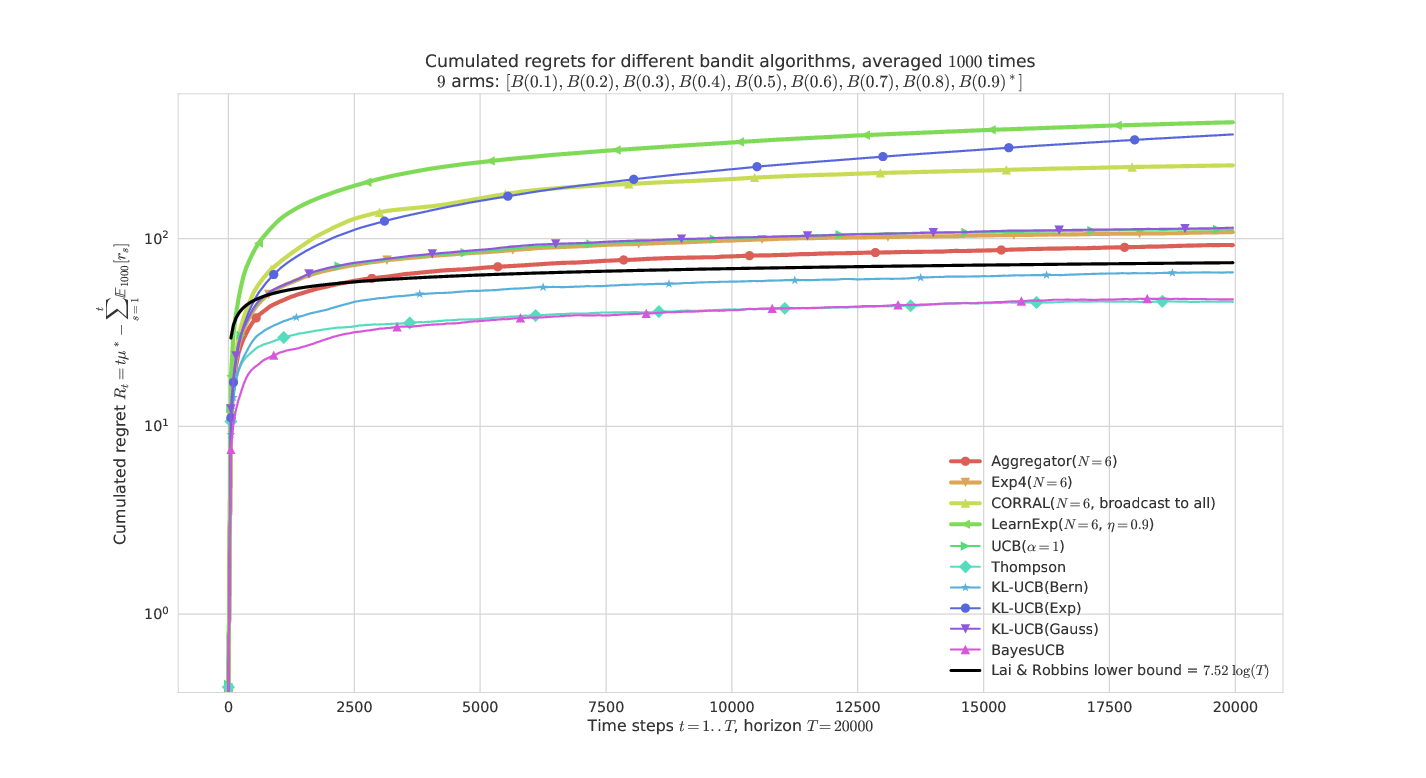
\includegraphics[width=1.00\linewidth]{plots/main_semilogy____env1-4_932221613383548446.pdf}
	\caption{\small On a ``simple'' Bernoulli problem (semi$\log$-$y$ scale).}
	\label{fig:EasyBernoulli}
\end{figure*}

\begin{figure}[b!]  % [htbp]
	\centering
	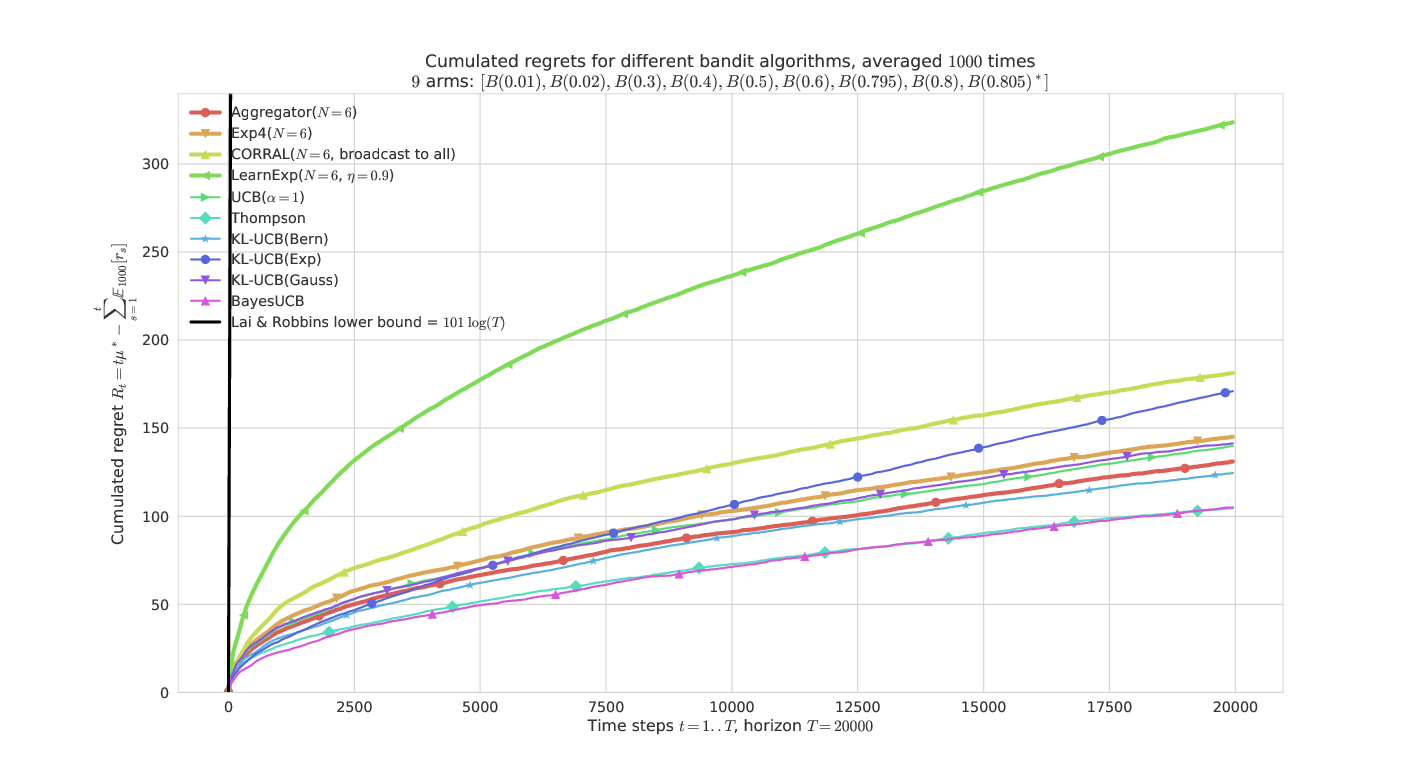
\includegraphics[width=1.04\linewidth,left]{plots/main____env2-4_932221613383548446.pdf}
	\caption{\small On a ``harder'' Bernoulli problem, they all have similar performances, except \LearnExp.}
	\label{fig:HardBernoulli}
\end{figure}
%
\begin{figure}[b!]  % [htbp]
	\centering
	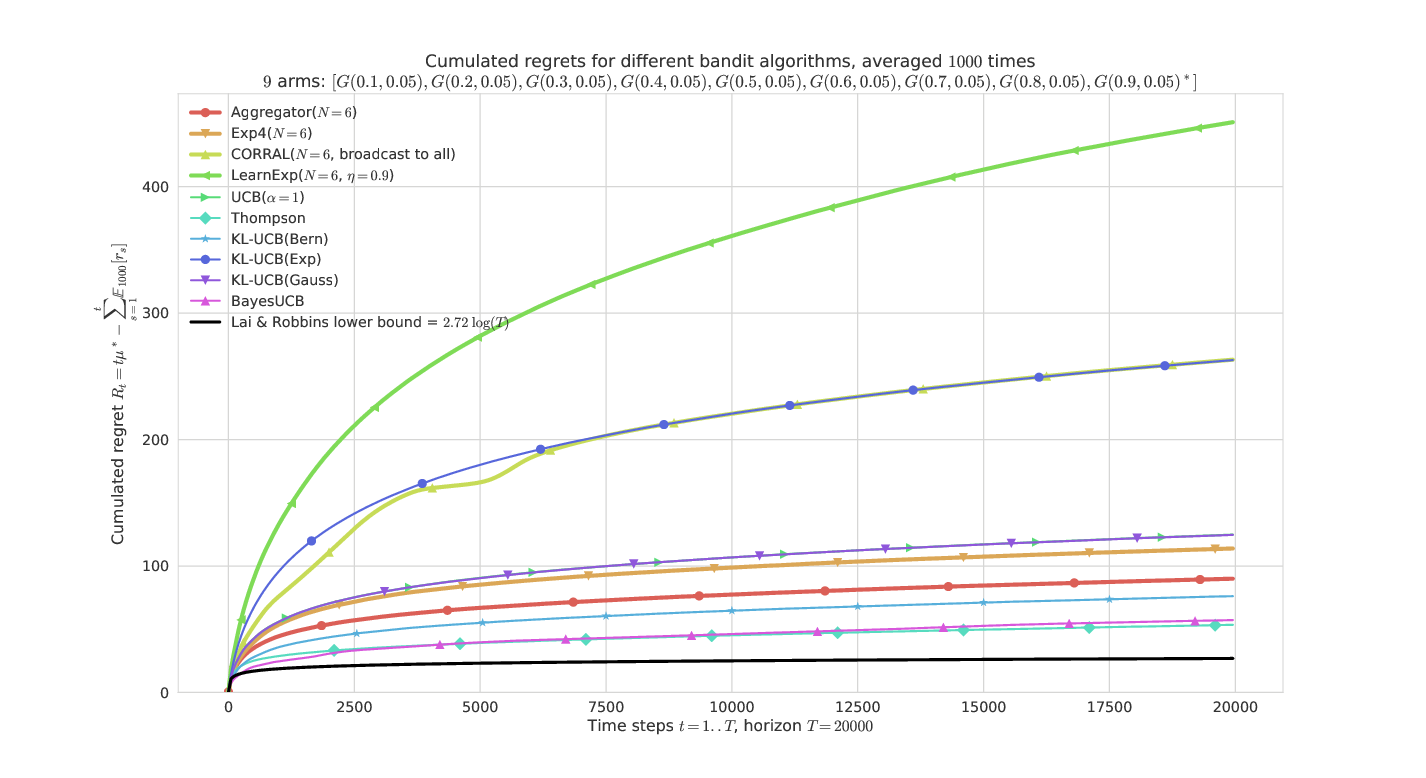
\includegraphics[width=1.04\linewidth,right]{plots/main____env3-4_932221613383548446.pdf}
	\caption{\small On an ``easy'' Gaussian problem, only \Aggr{} shows reasonable performances, thanks to BayesUCB and Thompson sampling.}
	\label{fig:EasyGaussian}
\end{figure}

% - explain the problem studied in the simulation
We focus on \emph{i.i.d.} MAB problems, with $K = 9$ channels\footnote{~Similar behaviors are observed for any not-too-large values of $K$, we tried up-to $K = 100$ and the same results were obtained.}.
% To give an idea, one simulation for one algorithm runs in about $40\;\mathrm{s}$ on a $4$-core Intel i5 Linux $64$-bits machine, with Python $3$ parallelized on $4$ cores, and in about $12\;\mathrm{min}$ for $N=8$ algorithms and their aggregation.},
For Bernoulli problem, the first one uses $\boldsymbol{\mu}=[0.1,\dots,0.9]$,
and the second one is divided in three groups:
2 very bad arms ($\mu = 0.01, 0.02$), 5 average arms ($\mu = 0.3$ to $0.6$) and 3 very good arms ($\mu = 0.78, 0.8, 0.82$).
The horizon is set to $T = 20000$ (but its value is unknown to all algorithms), and simulations are repeated $1000$ times, to estimate the expected regret.
%
This empirical estimation of the expected regret $R_T$ is plotted below, as a function of $T$, comparing some algorithms $\Alg_1,\dots,\Alg_N$ (for $N=6$), and their aggregation with \Aggr{} (displayed in orange bold).
% using the parameter-free learning rate sequence, $\eta_t := \log{N} / (t K)$.
The Lai \& Robbins' logarithmic lower-bound \cite{LaiRobbins85} is also plotted, and it is crucial to note that it is only asymptotic and to not be surprised by having regret curves smaller than the lower-bound (\eg, for the easier Bernoulli problem).
% (the continuous black
% \footnote{~These plots are best viewed in color.}
% line without marker).
% FIXME FIXME FIXME
%
Note that for each of the $1000$ simulations, we choose to generate all the rewards beforehand, \ie, one full matrix $(r_k(t))_{1\leq k \leq K, 1 \leq t \leq T}$ for every repetition, in order to compare the algorithms on the same realizations
% \footnote{Similar plots and similar results are obtained if this trick is not used, but it makes more sense to compare them against the same randomization.}
of the MAB problem.

We compare our \Aggr{} algorithm, % in 2 different versions,
as well as other aggregation algorithms, \ExpQ{},
% (two versions),
\CORRAL{} and \LearnExp{} (both with default parameters) \cite{Bubeck12,Agarwal16,Singla17}.
The aggregated algorithms consist in a naive uniform exploration (to have at least one algorithm with bad performances, \ie{} linear regret, but it is not included in the plots),
\UCB{} with $\alpha=1/2$, three \klUCB{} with Bernoulli, Gaussian and exponential $\kl$ functions, and BayesUCB and Thompson sampling with uniform prior.

Figures~\ref{fig:EasyBernoulli} and \ref{fig:HarderMixed} are in semi$\log$-$y$ scale, this helps to see that the best algorithms can be an \emph{order of magnitude} more efficient than the worst, and the \Aggr{} performs similarly to the best ones, when the other aggregation algorithms are usually amongst the worst.
Figure~\ref{fig:HarderMixed_semilogx} is in semi$\log$-$x$ scale to show that the regret of efficient algorithms are indeed logarithmic.

\begin{figure*}[h!]  % [htbp]
	\centering
	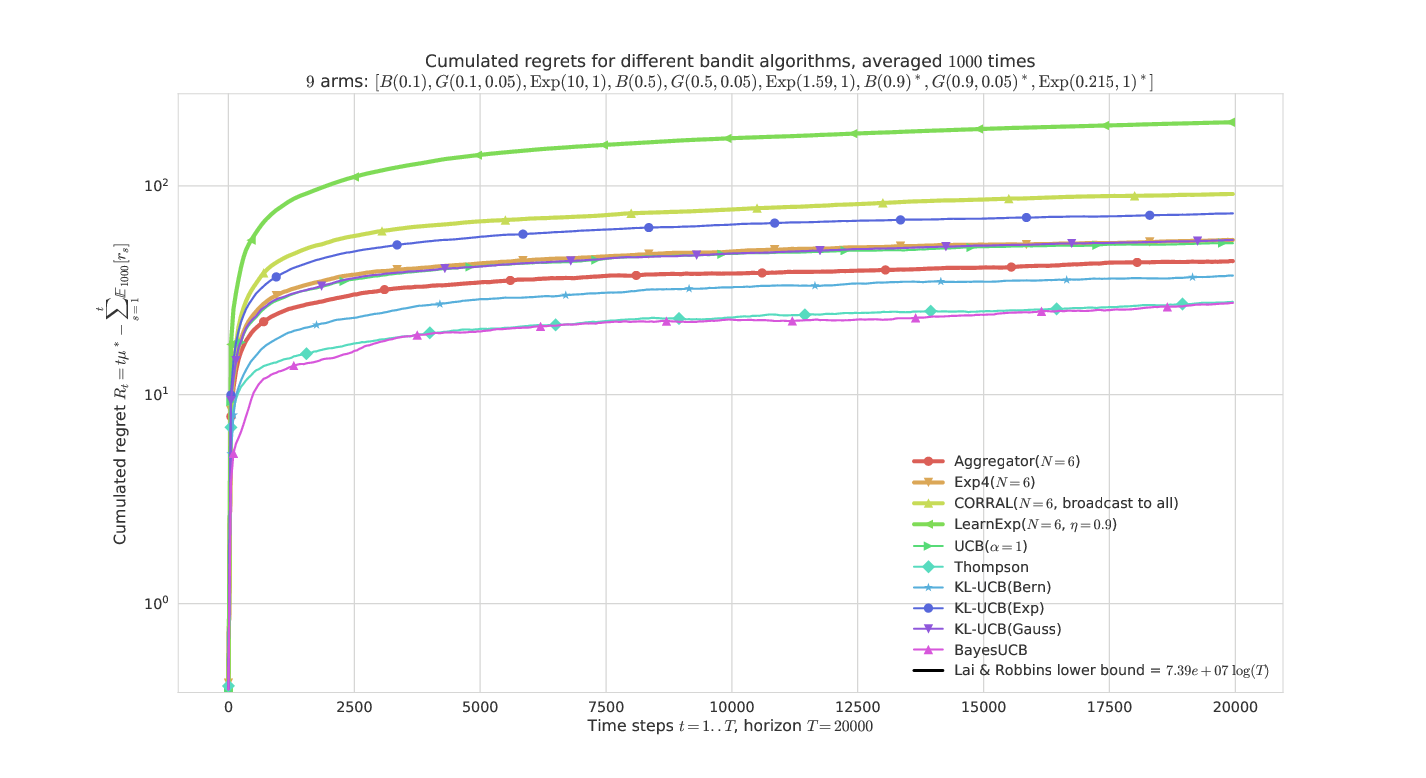
\includegraphics[width=1.05\linewidth,left]{plots/main_semilogy____env4-4_932221613383548446.pdf}
	\caption{\small On a harder problem, mixing Bernoulli, Gaussian, Exponential arms, with 3 arms of each types with the \emph{same mean}.}
	\label{fig:HarderMixed}
\end{figure*}

% \vspace*{-10pt}
\begin{figure}[b!]  % [htbp]
	% \centering
	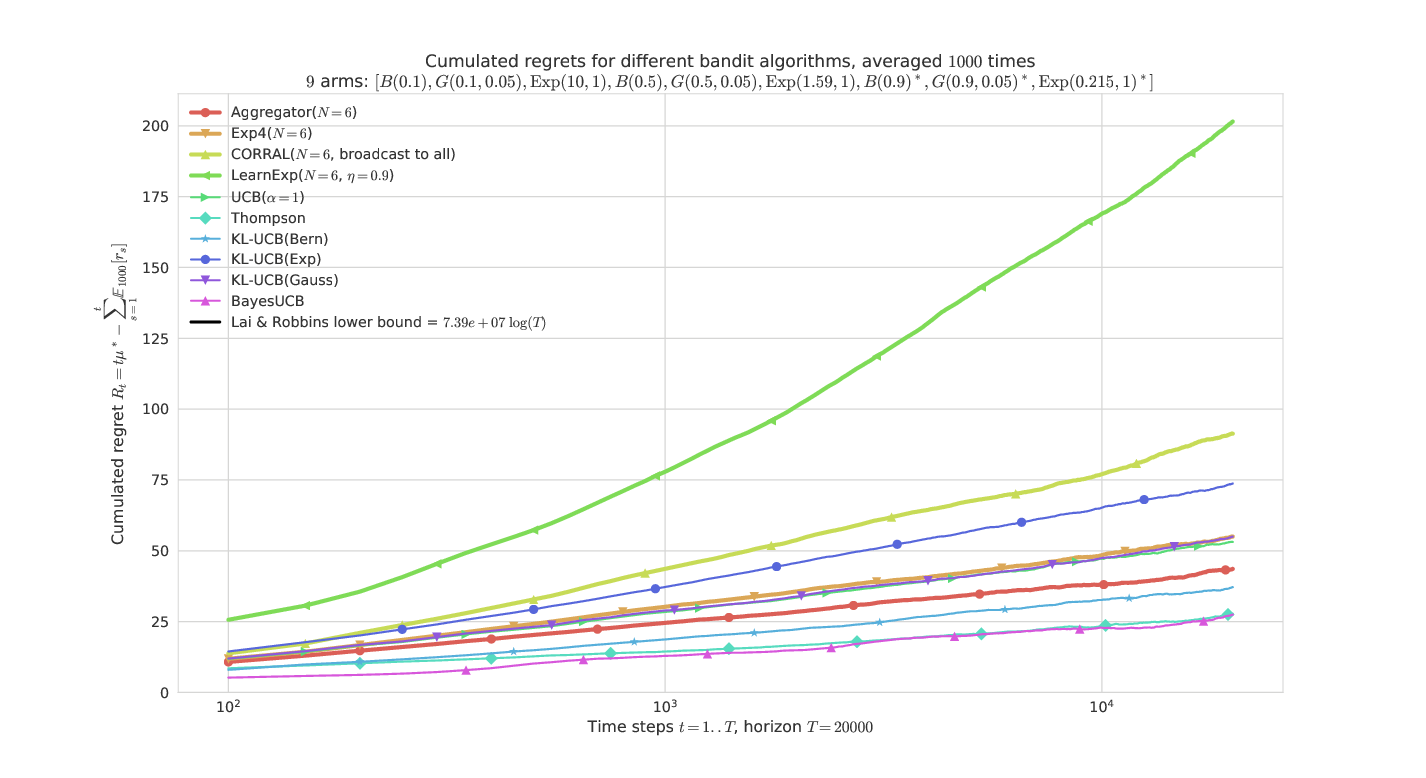
\includegraphics[width=1.07\linewidth,left]{plots/main_semilogx____env4-4_932221613383548446.pdf}
	\caption{\small The semi$\log$-$x$ scale clearly shows the logarithmic growth of the regret for the best algorithms and our proposal \Aggr, even in a hard ``mixed'' problem (\emph{cf}. Figure~\ref{fig:HarderMixed}).}
	\label{fig:HarderMixed_semilogx}
\end{figure}

For Bernoulli problems (Figures~\ref{fig:EasyBernoulli} and \ref{fig:HardBernoulli}), UCB with $\alpha=1/2$, Thompson sampling, BayesUCB and \klUCB{}$^+$ (with the binary $\kl$ function) all perform similarly, and \Aggr{} is found to be as efficient as all of them.
For Gaussian and exponential arms, rewards are truncated into $[0,1]$, and the variance of Gaussian distributions is fixed to $\sigma^2 = 0.05$ for all arms, and can be known to the algorithms (the \kl{} function is adapted to this one-dimensional exponential family).
%
Figure~\ref{fig:EasyGaussian} uses only Gaussian arms, with a large gap between their means and a relatively small variance, giving an ``easy'' problem.
%
And Figure~\ref{fig:HarderMixed} shows a considerably harder ``mixed'' problem, when the distributions are no longer in the same one-dimensional exponential family and so the Lai \& Robbins' lower-bound no longer holds (even if there still exists a lower-bound).

For each of the 4 problems considered, the \Aggr{} algorithm with default option (broadcast loss to all players) is the best of all the aggregation algorithms,
and its regret is very close to the best of the aggregated algorithms.
Especially in difficult problems with mixed or unknown distributions, \Aggr{} showed to be more efficient that \ExpQ{} and orders of magnitude better than the other reference aggregation algorithms \LearnExp{} and \CORRAL{} (see Figures~\ref{fig:HarderMixed} and \ref{fig:HarderMixed_semilogx}).


% - draw conclusions from these graphs

% - explain a little bit on non-Bernoulli problems

% - WHOO our algorithm is awesome!



% ----------------------------------------------------------------------
% \vspace*{50pt}
\section{Theoretical Guarantees}\label{sec:theory}

The \Aggr{} does not have satisfying theoretical guarantees in terms of regret $R_T$ yet, unlike many bandit algorithms.
%
Another notion, the \emph{adversarial regret}, denoted by $\overline{R_T}$,
measures the difference in terms of rewards,
between the aggregation algorithm $\Alg_{\mathrm{aggr}}$ and the best aggregated algorithm $\Alg_a$. This is in contrast with the (classical) regret, which measure the difference with the best fixed-arm strategy (Eq.~\eqref{eq:classicalregret}). Thus,  even if the aggregated algorithms have logarithmic (classical) regret, having an adversarial regret scaling as $\sqrt{T}$ does not permit to exhibit a logarithmic (classical) regret for the aggregation algorithm.
%
%
Under some additional hypotheses,
\cite[Theorem 4.2]{Bubeck12} proves that
\ExpQ{} satisfies a bound on adversarial regret, % $\overline{R_T}$
$\overline{R_T} \leq 2 \sqrt{T N \log{k}}$,
with the good choice of the learning rate sequence $(\eta_t)_{t \geq 1}$.
Our proposed algorithm follows quite closely the architecture of \ExpQ,
and a similar bound for \Aggr{} is expected to hold.
% this is left as a future work.
% For sake of conciseness, we cannot present a proof here.
%

This would be a first theoretical guarantee, but not satisfactory as simple algorithms like UCB have regrets scaling as $\log{T}$ \cite{Auer02,Bubeck12}, not $\sqrt{T}$.
%
Regret bounds in several different settings are proved for the \CORRAL{} algorithm \cite{Agarwal16}, but no logarithmic upper-bound can be obtained from their technique, even in the simplest setting of stochastic bandits.
%
However, \Aggr{} always seems to have a (finite-horizon) logarithmic regret in all the experiments we performed,
for both Bernoulli and non-Bernoulli problems (\eg, Gaussian, exponential and Poisson distributions).
Further theoretical developments are left as future work.

% ----------------------------------------------------------------------
%\newpage
\section{Conclusion}\label{sec:conclusion}

We presented the use of aggregation algorithms in the context of Opportunistic Spectrum Access for Cognitive Radio,
especially for the real-world setting of unknown problem instances,
when tuning parameters before-hand is no longer possible and an adaptive algorithm is preferable.
% - \ExpQ and \Aggr works fine
% Both algorithms \ExpQ{} and \Aggr{} have been detailed, and we explained why
Our proposed \Aggr{} was presented in details,
and we also highlighted its differences with \ExpQ.
% as well \color{red} as the intuition that it seems more suited for purely stochastic problems\color{black}.

% - \Aggr{} really help to select the best algorithm against a certain problem, on the fly without any prior knowledge of the problem neither any prior knowledge on which algorithms is the best
We realized experiments on simple MAB problems already used in the community of bandit algorithms for OSA \cite{Jouini10},
and the simulations results showed that \Aggr{} works as expected, being able to identify on the fly the best algorithm to trust for a specific problem.
Experiments on problems mixing different families of distributions were also presented, with similar conclusions in favor of \Aggr.
% - even in dynamic scenario ? FIXME check
It is not presented in this article, but our proposed algorithm also works well in dynamic scenarios, in which the distribution of the arms can change abruptly at some time,
and appears to be more robust than simple non-aggregated algorithms.
% FIXME is it the case ?

\ExpQ{} has theoretical guarantees in terms of adversarial regret, and even if the same result could hold for \Aggr, results in terms of classical regret are yet to be proved.
Empirically, \Aggr{} showed to always have a logarithmic
regret $R_T$ if it aggregates algorithms with logarithmic regrets (like UCB, \klUCB, Thompson sampling, BayesUCB etc).
It usually succeeds to be close to the best of the aggregated algorithms, both in term of regret and best arm pull frequency.
As expected, the \Aggr{} is never able to outperform any of the aggregated algorithms, but this was an over-optimistic goal.
%
What matters the most is that, empirically, \Aggr{} is able to quickly discover \emph{on the fly} the best algorithms to trust, and then performs almost as well as if it was following it from the beginning.

Our \Aggr{} algorithm can probably be rewritten as an Online Mirror Descent, as \ExpQ{} and \CORRAL,
but this does not appear useful as in the case of \CORRAL{}  the analysis cannot bring a logarithmic bound on the regret even by aggregating asymptotically optimal algorithms.
We will continue investigating regret bounds for \Aggr,
and other directions include possible applications to the non-stochastic case (\eg, rested or restless Markovian problems, like it was very recently studied in \cite{Luo17}).


% ----------------------------------------------------------------------

\newpage
\section{Acknowledgements}\label{sec:thanks}
% \begin{small}
	The authors would like to thank Odalric-Ambrym Maillard at Inria Lille,
	R{\'e}mi Bonnefoi and Quentin Bodinier at CentraleSup{\'e}lec Rennes, for fruitful discussions.
	% This work is supported by the French Agence Nationale de la Recherche (ANR), under grant ANR-16-CE40-0002 (project BADASS)
% \end{small}


%\newpage


% ----------------------------------------------------------------------

% \begin{footnotesize}  % XXX
	% \nocite{*}  % XXX remove to hide references not cited!
	% \bibliographystyle{alpha}
	% \bibliographystyle{naereen}  % XXX use alpha if any issue occurs with my custom theme
	\bibliographystyle{ieeetr}
	\bibliography{IEEE_WCNC__2018__Paper__Lilian_Besson__07-17}

	% \begin{small}
		\hr{}
		\emph{Note:} the source code (Python $2$ or $3$) used for the simulations and the figures is not yet open-sourced, but is available upon request,
		and a full documentation is available at
		% More details at
		\texttt{http://banditslilian.gforge.inria.fr/}.
		% \texttt{https://Naereen.GitHub.io/AlgoBandits}.
	% \end{small}
	% \end{footnotesize}  % XXX

\end{document}
